%This work is licensed under the Creative Commons License Attribution 4.0 International (CC-BY 4.0)
%https://creativecommons.org/licenses/by/4.0/legalcode
\documentclass[rgb]{standalone}
\usepackage{tkz-euclide}
\definecolor{myorange}{hsb}{0.0833, 1, 0.8}
\definecolor{mygreen}{hsb}{0.3333, 1, 0.8}
\definecolor{myblue}{hsb}{0.5833, 1, 0.8}
\definecolor{mymagenta}{hsb}{0.8333, 1, 0.8}
\begin{document}
	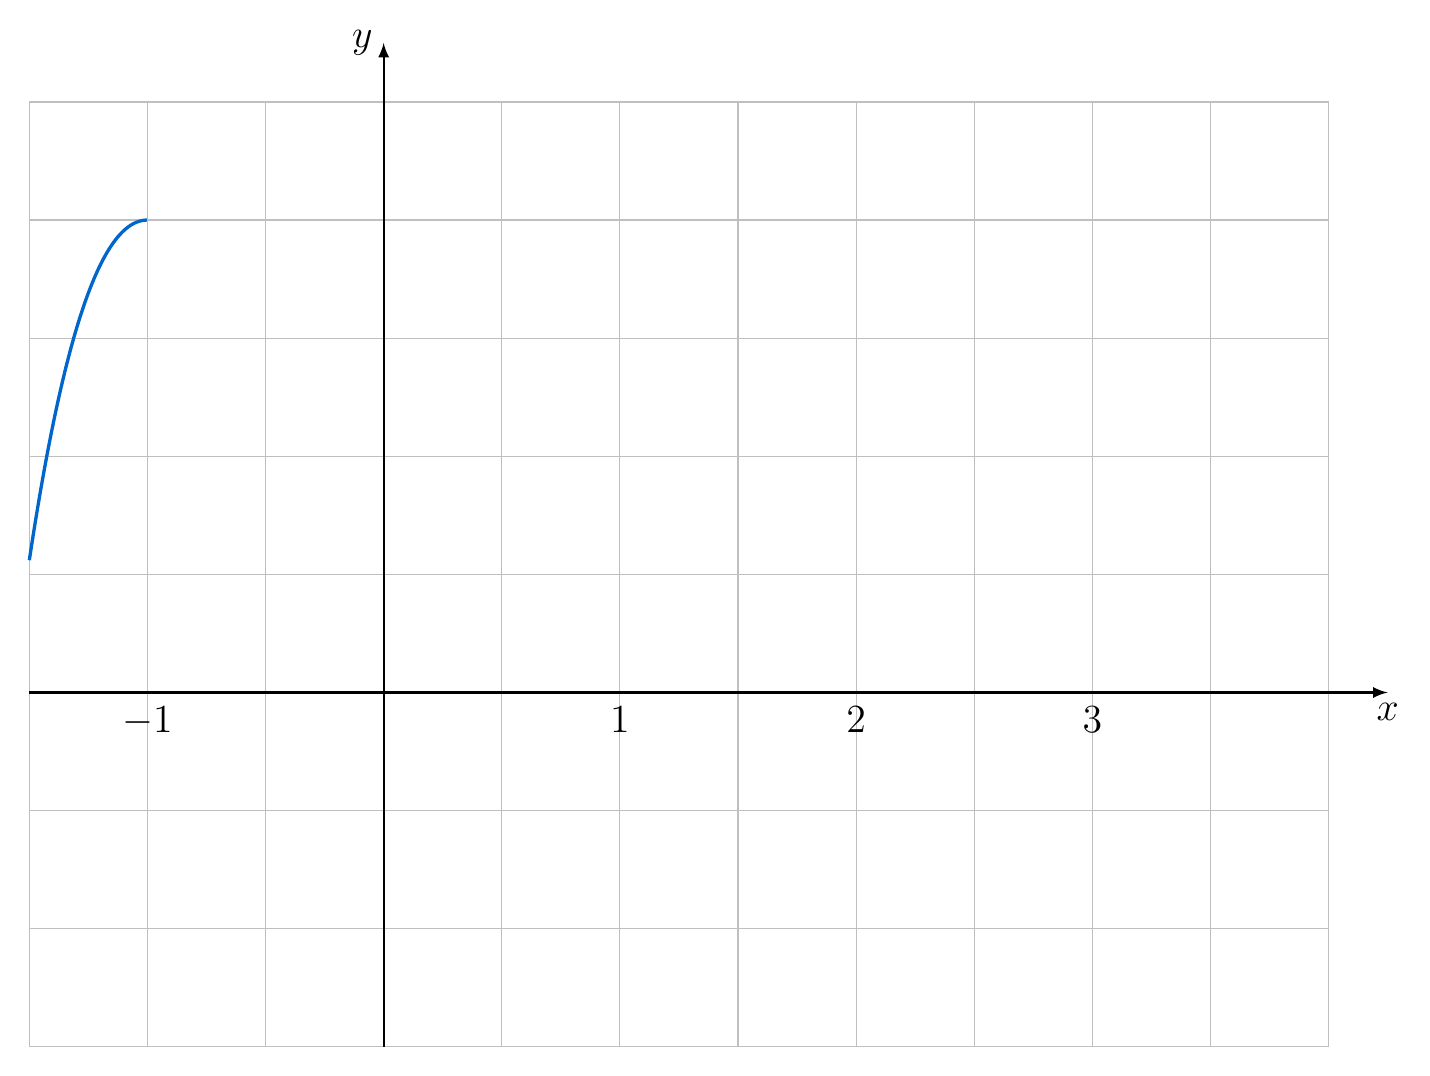
\begin{tikzpicture}[scale=1.5, font=\Large]
		% Coordinate system
		\tkzInit[xmin=-3,xmax=8,ymin=-3,ymax=5]
		\tkzGrid[color=lightgray]
		\tkzDrawX[thick]
		\tkzDrawY[thick]
		\draw[very thick,domain={-1.5}:{-1}, samples=200, smooth, variable=\x,myblue] plot ({2*\x}, {240/229*(1/10*\x*\x*\x*\x*\x-3/4*\x*\x*\x*\x+4/3*\x*\x*\x+3/2*\x*\x-9/2*\x)});
		% Labels
		%\node[left=0.5mm] at (0,4){$2$};
		%\node[left=0.5mm] at (0,2){$1$};
		%\node[left=0.5mm] at (0,-2){$-1$};
		\node[below=0.5mm] at (-2,0){$-1$};
		\node[below=0.5mm] at (2,0){$1$};
		\node[below=0.5mm] at (4,0){$2$};
		\node[below=0.5mm] at (6,0){$3$};
	\end{tikzpicture}	
\end{document}